\documentclass{article}

\usepackage{amsmath, amssymb, amscd}
\usepackage{url}
\usepackage{graphicx}
\usepackage{amsthm}
\usepackage[all]{xy}
\usepackage{multirow}
\usepackage{subfigure}



% Puts more text on each page
\addtolength{\topmargin}{-.75in}
\addtolength{\textheight}{1.5in}
\addtolength{\oddsidemargin}{-.5in}
\addtolength{\textwidth}{1.0in}


\title{\vspace{60 mm}SwarmVis - A Tool For Visualizing Swarm Systems\\User Guide}
\author{Don Miner and Niels Kasch}
\date{December 5, 2008}

\begin{document}
\maketitle
\pagebreak
\tableofcontents

\pagebreak
\section{Introduction}

This document describes the user interface of SwarmVis, a tool that allows swarm researchers to visualize swarm systems in two and three dimensional space. The tool enables researchers to track swarms and agents of a swarm in a continuous time simulation. It is the goal of the toolkit to provide insight in the development and evolution of swarms systems by allowing researchers to apply agent and swarm level visualization while browsing back and forth through the discrete time steps in the lifetime of a swarm.

\section{The User Interface}

SwarmVis consists of graphical user interface (GUI) in the form of a window embedded with control and rendering widgets. 
The main window is divided into three major components:
\begin{enumerate}
\item a tab control - allowing access to various visualizations and settings (Figure \ref{tabcontrol})
\item a playback control - controlling the progression of time frames(Figure \ref{playbackcontrol})
\item a rendering window - responsible for rendering the visualizations (Figure \ref{renderwindow})
\item a menu bar - allowing the loading of datasets (Figure \ref{filemenu})
\end{enumerate}

%%%%%%%%%%%%%%%%%%%%%%%%%%%%%
\begin{figure}[htp]
     \centering
     \subfigure[The Tab Control gives access to the various visualization capabilities in SwarmVis. The image illustrates the \textit{Agents Tab} where the color and size of individual agents can be manipulated.]{
      \label{tabcontrol}
      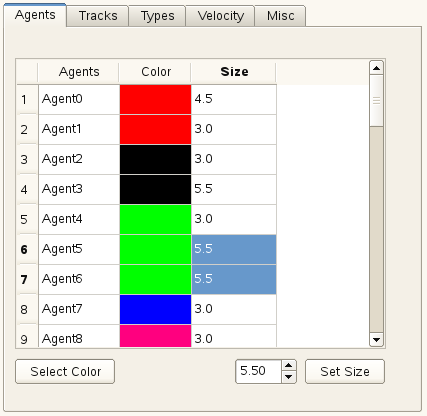
\includegraphics[scale=0.4]{images/tabcontrol.png}
     }
     \hspace{.3in}
     \subfigure[The Render (OpenGL) window where all visualizations are rendered. A typical visualization includes a bounding box for reference.]{
      \label{renderwindow}
     	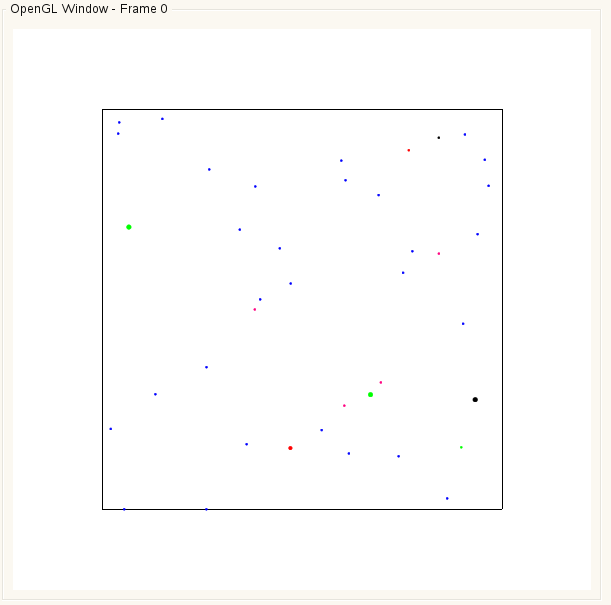
\includegraphics[scale=0.3]{images/renderwindow.png}
     }
     \\ 
     \hspace{.3in}
     
    \subfigure[The Playback Control enables the \textit{browsing} through the visual representation of a swarm dataset. The \textit{Play} button starts a continuous time simulation of a dataset whereas the \textit{slider} allows for the rewinding and fast-forwarding of the simulation.]{
      \label{playbackcontrol}
      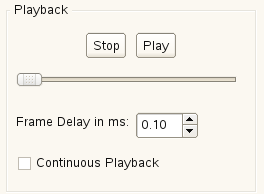
\includegraphics[scale=0.5]{images/playbackcontrol.png}
     }     
     \hspace{.3in}
    \subfigure[The File Menu allows for the loading of datasets. The Settings Menu can be used to load/save user specific settings for a particular visualization.]{
      \label{filemenu}
      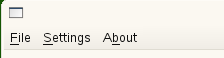
\includegraphics[scale=0.7]{images/filemenu.png}
     }
     
    \caption{The SwarmVis User Interface.}
     \label{interface}
\end{figure}


%%%%%%%%%%%%%%%%%%%%%%%%%%%%%
\subsection{The Tab Controls}

\subsubsection{The Agents Tab}
The \textit{Agents} tab facilitates selection of features for individual agents. Using the \textit{Agents} tab, a user is able to manipulate the visual representation of an agent, such as color and size. To change the color of an agent, select the agents followed by pressing the \textit{Select Color} button. A color dialog is displayed facilitating the selection of an RGB color. The size of an agent can be adjusted via a \textit{spinbox} and the \textit{Set Size} button. Multiple agents can be selected by (1) dragging the mouse over multiple agents, (2) pressing and holding the \texttt{CTRL} key on the keyboard while clicking on individual agents in the list (individual selection) and (3) pressing and holding the \texttt{Shift} key (continuous selection).

\subsubsection{The Tracks Tab}
The \textit{Tracks} tab allows a user to track the path of selected agents over the entire simulation. Tracks can be visualized using the specific color of an agent or a selected general color for all agents. Visualizing tracks with agent specific colors allows users to provide an instant overview of an agents past and future positions. This visualization technique is particularly useful during ``freeze frame'' analysis. Select an agent to visualize its track. Multiple selections are allows similarly to selecting agents on the \textit{Agents} tab.

Tails can be enabled via the \textit{tails spinbox} provided on the tab. The tail view shows the position of all agents in previous time steps. The length of the trail can be adjusted by increasing the value of the spinbox. Tails progressively fade according to the tails temporal distance in relation to the current time step. 

\subsubsection{The Types Tab}
The \textit{Types} tab shows an overview of the different types of agents and provides a facility to distinguish the types according to selected colors. Particular datasets can annotate the data with several types of agents. Each agent type may operate according to different rules and hence behaves differently. The \textit{Types} tab facilitates visual distinction of types which makes the task of tracking types easier for a user.

\subsubsection{The Velocity Tab}
The \textit{Velocity} tab implements functionality to visualize the velocity of the agents. A rainbow scale shown on the tab, maps color according to speed. When enabled the agents and/or agent tracks/trails change color according to the speed an agent travels. It is noteworthy that track segments are colored according to the speed at which the agent was traveling for a particular segment.

\subsubsection{The Misc Tab}
The \textit{Misc} tab provides additional functionalities to control the visualization. Via a \textit{checkbox}, a user can enable or disable the bounding box surrounding the visualization. The bounding box can be useful in providing context when the view window is rotated or its size is changed. OpenGL depth checking can be enabled via the respective checkbox. Depth checking is a feature of OpenGL to access the depth of a pixel from the viewing plane. This allows a pixel at a certain depth to assess whether or not other pixels overlay the current viewport.

\subsection{The Playback Control}

The playback control functionality is comparable to a standard media player. It allows for the playing, pausing, rewinding and fast-forwarding of the swarm animation in the render window. A slider bar is provided to give an overview and control over the currently displayed frame. Advancing and moving back the slider skips to future and past time frames, respectively.

\subsection{The Render/OpenGL Control}

The render/OpenGL window displays the frames of the swarm animation. Since SwarmVis supports 3D visualizations of swarm systems, a bounding box for providing orientation is 3D space can be enabled via the \textit{Misc Tab}. The render window supports zooming and rotating the view. The zoom feature can be activated by hovering a mouse over the render window and utilizing the scroll wheel on a mouse (scroll up = zoom in; scroll down = zoom out). Rotation of the view can be accomplished by clicking the left or right mouse button while simultaneously moving the mouse. The left mouse button activates rotation over the x and y axes, whereas the right mouse button activates rotation over the x and z axes.

\subsection{The Menu Bar}

The menu bar consists of three components, namely the \textit{File}, \textit{Settings} and \textit{About} menus.
The \textit{File} menu allows a user to (1) exit the application and (2) load swarm datasets to be visualized. The swarm dataset are loaded through an information file (the structure of the information file is described in Section \ref{fileformat}) which can be selected via an open file dialog.

The \textit{Settings} menu enables a user to load and save the settings (i.e. color and size of agents, time frame displayed in the render window and state of all check boxes and selected agents) for a visualization. \textit{Save Settings} stores all settings in a file specified by the user. \textit{Load Settings} restores the settings from a selected file. This feature permits a user to save and restore ``interesting'' situations or occurrences in a visualization.

The \textit{About} menu simply displays information about the authors of SwarmVis.


\section{Compiling and Running}
SwarmVis is a cross-platform tool
and is intended to run on Unix-like systems, such as Mac OS X and GNU/Linux, as well as Microsoft Windows.
The source code is available at:\begin{quote}\texttt{http://code.google.com/p/swarm-vis/}\end{quote}
The following programs are required to compile SwarmVis from source:
\begin{itemize}
\item Qt 4.2\footnote{Qt is an open source cross-platform application framework. It is available at http://trolltech.com/downloads}
\item gcc/g++ 4.2.2
\item make
\end{itemize}
Note that some libraries from Qt4.2 may be needed to run the SwarmVis binary.
We have tested SwarmVis on Mac OSX 10.5 and openSUSE Linux 11.

Run \texttt{qmake}, and then \texttt{make}, both in SwarmVis' root directory (where the file \texttt{swarmvis.pro} is located), to compile SwarmVis.
A binary will be created in the \texttt{bin/} directory. Execute this binary to run SwarmVis.

\section{Data File Format}\label{fileformat}
SwarmVis requires a specific format for data sets that are to be loaded. The agents' position data is segmented into
separate files that each represent a single time step. These files contain space-delimited data, with
each row representing an agent. For example, a swarm system with 100 agents depicted over 500 time steps
will have 500 files in a folder, each with 100 lines of text.

Each row entry in a file must follow a specific format. The first two or three  columns (depending on dimensionality) are the
position data $(X, Y)$ or $(X, Y, Z)$, respectively. The last column is reserved for the group label, which may be used to pass
group membership data to SwarmVis.
For example, a well-formed entry that conveys a three-dimensional position with group information could be:
\begin{quote}
\texttt{10.15 5.24 84.85 Corner}
\end{quote}
The order of the listing of agents in each file must be consistent.
That is, the $k^{th}$ entry in one file and the $k^{th}$ entry in another file must represent the same agent.

A plain-text information file containing important meta-data must accompany the frame files in the same directory.
The following variables must be defined (i.e., \texttt{VARNAME = VALUE}) in this file in order for the data to be loaded appropriately:
\begin{itemize}
\item \texttt{DIMENSIONS} (\texttt{2} or \texttt{3})
\item \texttt{AGENTS} (the number of agents)
\item \texttt{FRAMES} (the number frames/time steps)
\item \texttt{RANGEX} (the maximum X value)
\item \texttt{RANGEY} (the maximum Y value)
\item \texttt{RANGEZ} (the maximum Z value)
\item \texttt{AGENTTYPES} (\texttt{1} to track agent types, \texttt{0} if not)
\end{itemize}
At the bottom of this file, the keyword \texttt{FILES} must appear, followed by a list of frame files, in ascending
temporal order.
The number of files listed here must equal the number specified by the \texttt{FRAMES} variable.
Also, the number of lines in every file must match the number specified by the \texttt{AGENTS} variable.
To load a data set in the SwarmVis application, navigate to ``Load Data" and select the info file.

A sample info file for a 150 agent three-dimensional swarm over the course of 446 frames:


\begin{verbatim}
     DIMENSIONS = 3
     AGENTS = 150
     FRAMES = 446
     RANGEX = 600
     RANGEY = 600
     RANGEZ = 600
     AGENTTYPES = 1
     FILES
     frame000001.txt
     frame000002.txt
     frame000003.txt
     frame000004.txt
     frame000005.txt
     frame000006.txt
     ...
     frame000442.txt
     frame000443.txt
     frame000444.txt
     frame000445.txt
     frame000446.txt
\end{verbatim}



%\bibliographystyle{plain-annote}

%\bibliography{userguide}

\end{document}
